\chapter{Arquitectura y diseño técnico}\label{disarqtecnica}

\section{Arquitectura de la aplicación}

\begin{figure}[h]
    \centering
    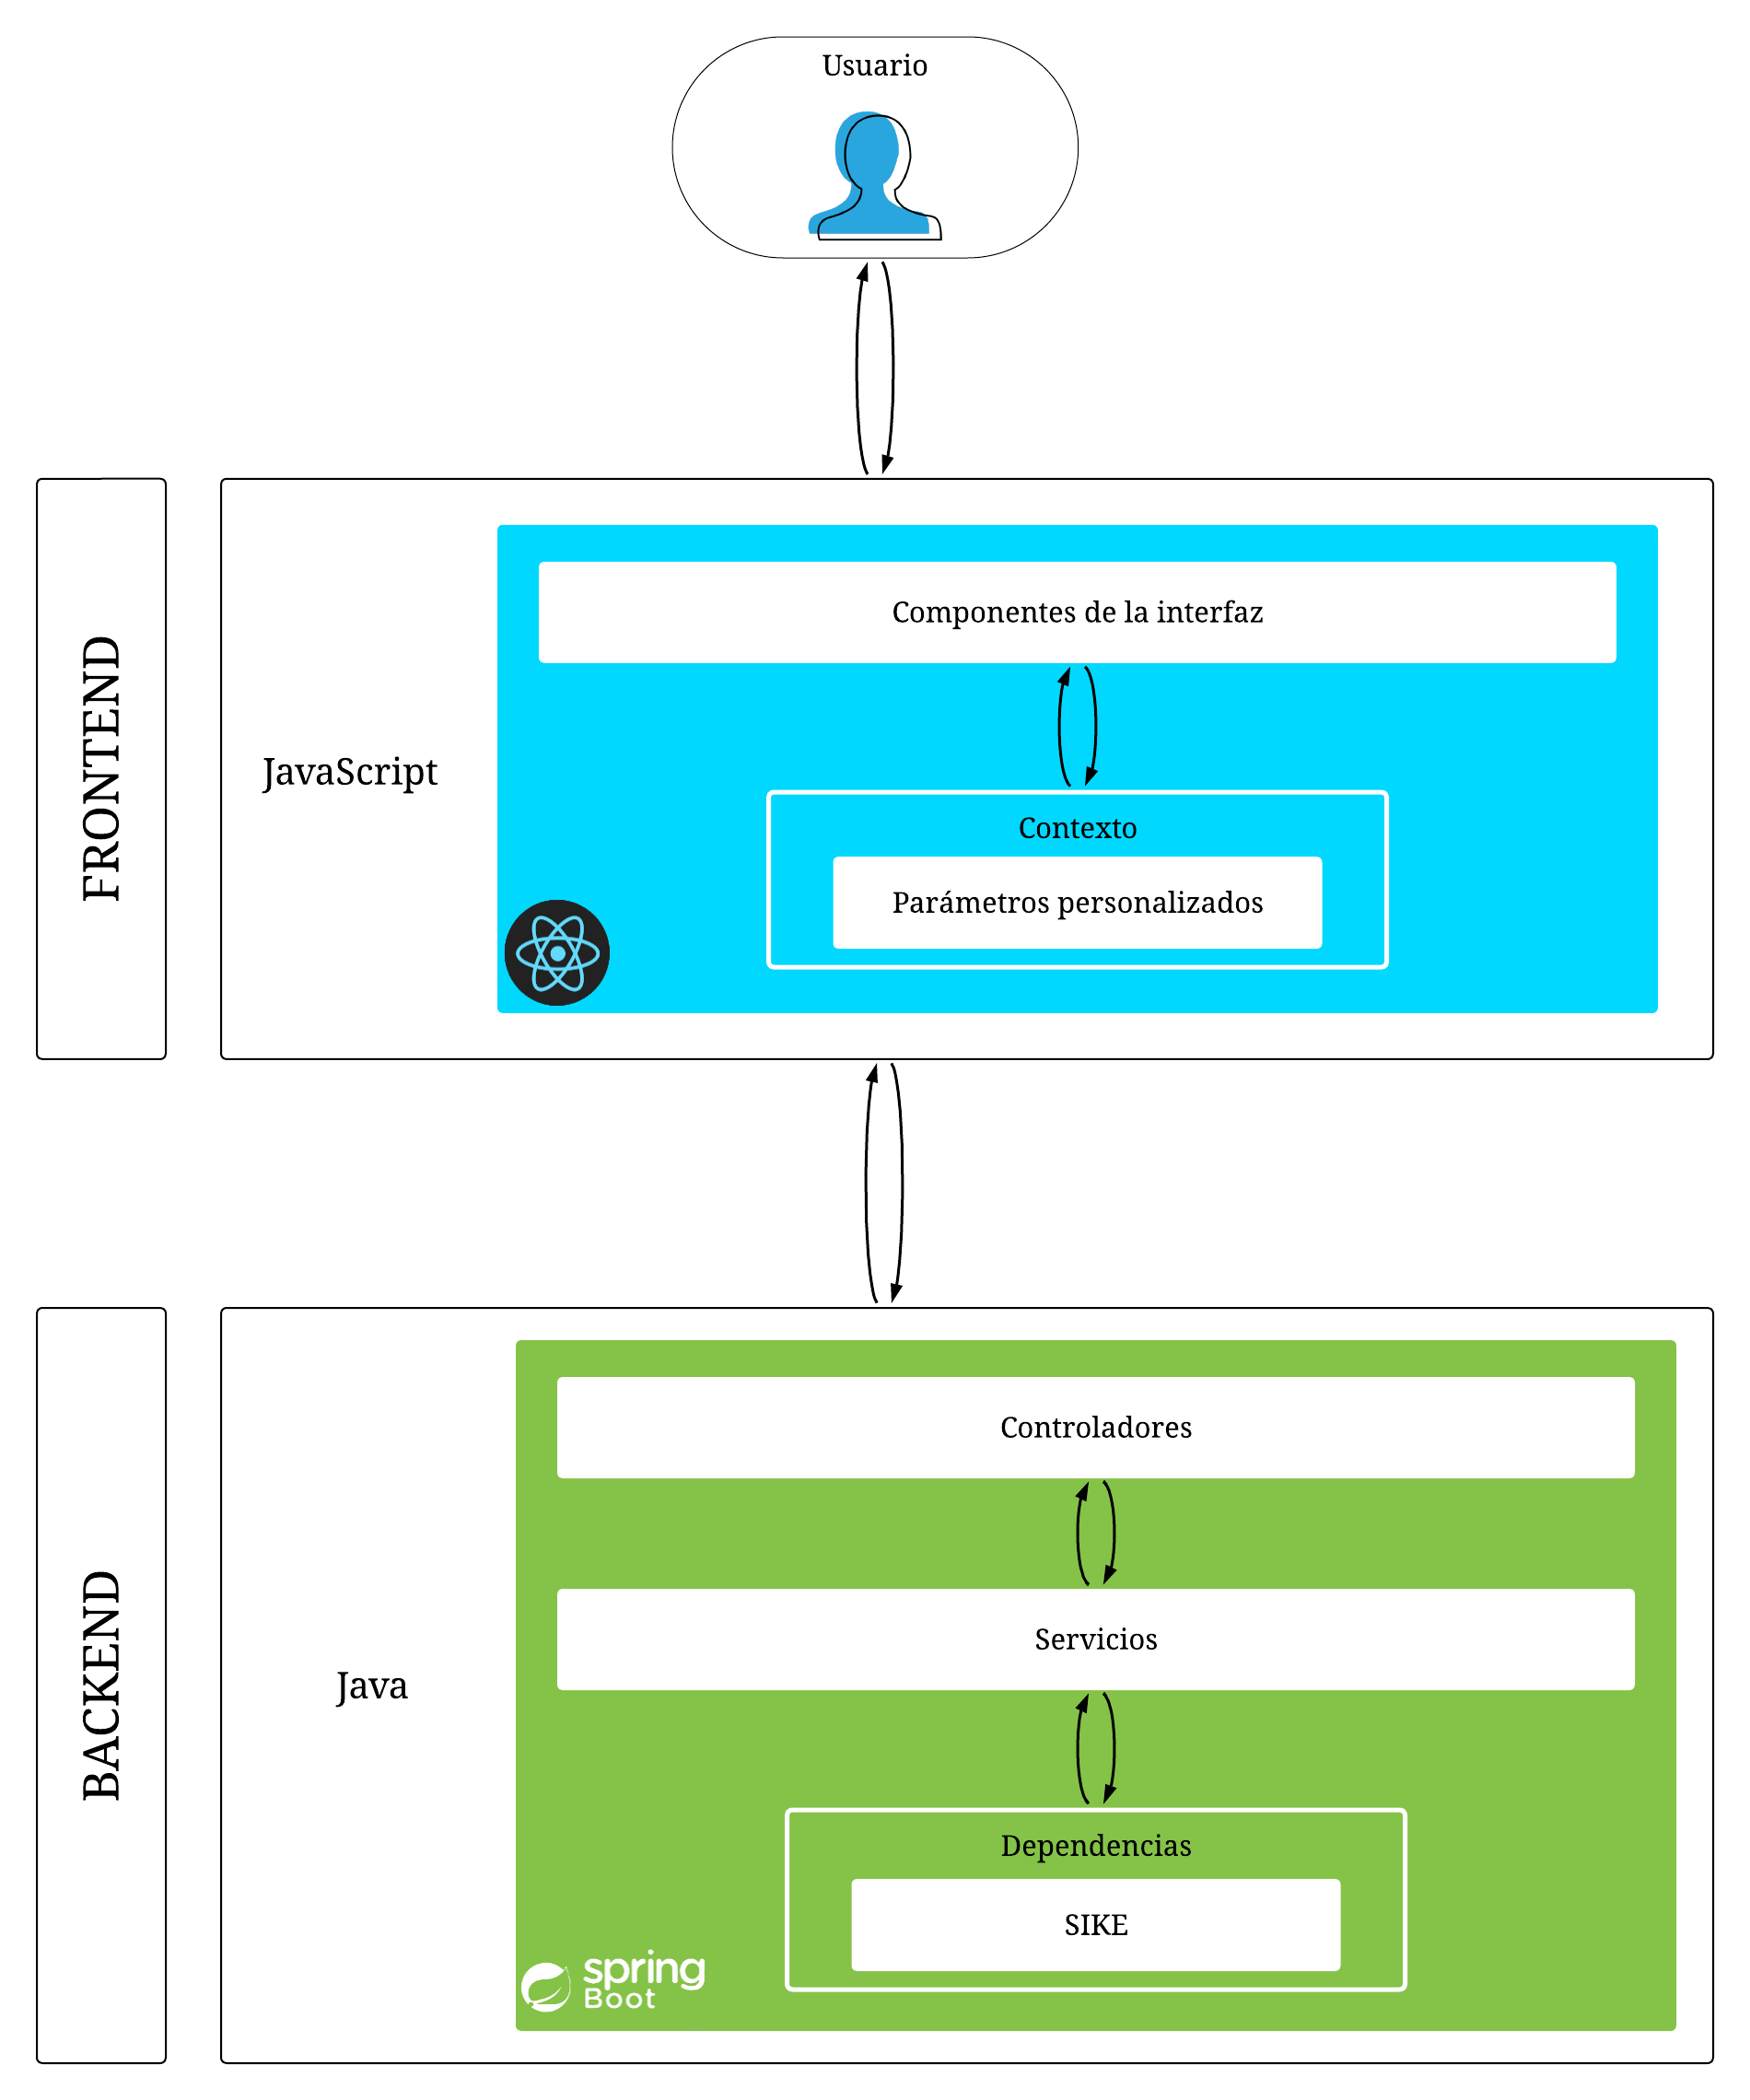
\includegraphics[width=0.75\linewidth]{img/Diagrama de capas.png}
    \caption{Diagrama de la estructura de la aplicación}
    \label{fig:diagrama-capas}
\end{figure}

Puesto que nos hemos visto obligados a utilizar tecnologías diferentes para la capa de presentación y la de lógica, tal y como exponemos en el capítulo \ref{tecnologias} decidimos implementar una arquitectura en capas tal y como queda reflejado en el anterior diagrama.

De esta forma reducimos el acoplamiento y aumentamos la cohesión, al separar las responsabilidades del proyecto. Además, permite utilizar cada capa casi como una unidad independiente.

\section{Diseño de la aplicación}

A continuación, veremos los patrones de diseño que hemos seguido a la hora de desarrollar la aplicación.

\subsection{Patrones creacionales}

En referencia a los patrones utilizados a la hora de crear objetos.

\subsubsection{Builder}

El patrón que hemos utilizado es el de Builder, que permite abstraer la creación de un objeto complejo, como es la entidad sobre la que reposa nuestra implementación, ya que para crear el mensaje cifrado y el mensaje descifrado hace falta lógica específica.

De esta forma conseguimos atomizar el proceso de creación para evitar que cualquier otro proceso del proyecto pueda interferir en él.


\subsection{Patrones estructurales}

En relación a la forma de ordenar internamente el proyecto.

\subsubsection{Module}

A la hora de implementar la vista de presentación de protocolo, en vez de duplicar la lógica de la presentación para cada protocolo, lo que hemos hecho ha sido crear una vista genérica de protocolo \verb|ProtocolView| que llama a las presentaciones específicas. Esta vista general agrupa los componentes marco de las presentaciones, el reproductor y los componentes genéricos inicial y final.

\subsubsection{Objeto Compuesto}\label{objeto-compuesto}

La presentación de los protocolos funciona como una presentación genérica de diapositivas, sin embargo, estas "diapositivas" son componentes React con sus estilos adicionales. Aunque algunas de ellas son tan sencillas como una imagen y algo de texto, hay otras que contienen componentes animados o incluso su propia lógica. Es por esto que decidimos tratar cada protocolo como una presentación al completo, importando a la vista \verb|ProtocolView| previamente definida una lista con todos los componentes para que esta tan sólo itere sobre ella. De esta forma conseguimos simplificar la lógica general a la vez que mantenemos cada paso de la presentación autocontenido.


\subsection{Patrones de comportamiento}

Aquellos que tratan la interacción y responsabilidades entre clases y módulos

\subsubsection{Método Plantilla}

Como hemos mencionado en el patrón \ref{objeto-compuesto} Objeto Compuesto, hay pasos que tienen una lógica interna. Esta lógica queda autocontenida en la subclase y no afecta en ningún momento al reproductor automáticos de las diapositivas.

\subsubsection{Iterador}

Como explicábamos en el patrón de \ref{objeto-compuesto} Objeto Compuesto, tratamos las explicaciones de cada protocolo como una lista de componentes React para simplificar su uso.

\subsubsection{Estado}

Para que los parámetros y valores de ejemplo de SIKE se mantengan constantes a lo largo de la explicación y para que cualquier cambio se refleje a nivel global, utilizamos los contextos que proporciona React, de forma que cuando el usuario introduce un mensaje personalizado o vuelve a generar el secreto compartido, estos valores se reflejen en los pasos siguientes para que el usuario vea una implementación real del protocolo.